%%%%%%%%%%%%%%%%%%%%%%%%%%%%%%%%%%%%%
%                                   %
% Compile with XeLaTeX and biber    %
%                                   %
% Questions or comments:            %
%                                   %
% joshua dot mcneill at uga dot edu %
%                                   %
%%%%%%%%%%%%%%%%%%%%%%%%%%%%%%%%%%%%%

\documentclass{beamer}
  % Read in standard preamble (cosmetic stuff)
  %%%%%%%%%%%%%%%%%%%%%%%%%%%%%%%%%%%%%%%%%%%%%%%%%%%%%%%%%%%%%%%%
% This is a standard preamble used in for all slide documents. %
% It basically contains cosmetic settings.                     %
%                                                              %
% Joshua McNeill                                               %
% joshua dot mcneill at uga dot edu                            %
%%%%%%%%%%%%%%%%%%%%%%%%%%%%%%%%%%%%%%%%%%%%%%%%%%%%%%%%%%%%%%%%

% Beamer settings
% \usetheme{Berkeley}
\usetheme{CambridgeUS}
% \usecolortheme{dove}
% \usecolortheme{rose}
\usecolortheme{seagull}
\usefonttheme{professionalfonts}
\usefonttheme{serif}
\setbeamertemplate{bibliography item}{}

% Packages and settings
\usepackage{fontspec}
  \setmainfont{Charis SIL}
\usepackage{hyperref}
  \hypersetup{colorlinks=true,
              allcolors=blue}
\usepackage{graphicx}
  \graphicspath{{../../figures/}}
\usepackage[normalem]{ulem}
\usepackage{enumerate}

% Document information
\author{M. McNeill}
\title[FREN2001]{Français 2001}
\institute{\url{joshua.mcneill@uga.edu}}
\date{}

%% Custom commands
% Lexical items
\newcommand{\lexi}[1]{\textit{#1}}
% Gloss
\newcommand{\gloss}[1]{`#1'}
\newcommand{\tinygloss}[1]{{\tiny`#1'}}
% Orthographic representations
\newcommand{\orth}[1]{$\langle$#1$\rangle$}
% Utterances (pragmatics)
\newcommand{\uttr}[1]{`#1'}
% Sentences (pragmatics)
\newcommand{\sent}[1]{\textit{#1}}
% Base dir for definitions
\newcommand{\defs}{../definitions}


  % Packages and settings

  % Document information
  \subtitle[Révision, examen final]{Révision de l'examen final}

\begin{document}
  % Read in the standard intro slides (title page and table of contents)
  \begin{frame}
    \titlepage
    \tiny{Office: % Basically a variable for office hours location
Gilbert 121\\
          Office hours: % Basically a variable for office hours
 lundi, mercredi, vendredi 10:10--11:10
}
  \end{frame}

  \begin{frame}{Le jeu}
    \alert{Le prix:} 2\% sur l'examen pour le/la gagnant/e, 1\% pour la deuxième place \\
    \vspace{0.25cm}
    \alert{Les règles:}
    \begin{enumerate}
      \item Pose une question concernante l'examen
      \begin{itemize}
        \item Si personnne ne peut y répondre $\to$ +1
        \item Si quelqu'un peut y répondre $\to$ +0
        \item On a \alert{30 secondes} pour répondre
      \end{itemize}
      \item Si tu poses une question déjà posée $\to$ +0
      \item Si tu poses une question qui ne concerne pas l'examen $\to$ +0
    \end{enumerate}
    \vspace{0.25cm}
    \alert{Indice:} Tu peux poser la question en anglais, mais si tu poses la question \emph{en français}, seulement ceux qui la comprendre peut y répondre.
  \end{frame}

  %% Vocab to keep in mind -------------------------------------------------------------------------------------
  % body parts and health
  % environment
  % volunteer work
  % technology
  % activities
  % tourist sites and travel
  % buildings and rooms
  % directions
  % weather
  %% ------------------------------------------------------------------------------------------------------------

  \begin{frame}{Le subjonctif ou non?}
    \begin{enumerate}
      \item Jean est content que nous \underline{\uncover<2->{allions}} (aller) au village perché aujourd'hui.
      \item C'est dommage que tu \underline{\uncover<3->{aies}} (avoir) mal au ventre.
      \item Il faut \underline{\uncover<4->{prendre}} (prendre) ce vélo-ci et aller tout droit pour arriver à la cathédrale.
      \item Vous êtes travailleur, donc il est utile que vous \underline{\uncover<5->{vous rappeliez}} (se rappeler) votre valeur.
      \item Je crois que l'auberge \underline{\uncover<6->{est}} (être) à Bruxelles près de l'aéroport.
      \item Elle est gênée de \underline{\uncover<7->{faire}} (faire) du cheval quand il fait froid.
      \item Jenna est gênée que Jenna \underline{\uncover<8->{fait}} (faire) du cheval quand il fait frais.
    \end{enumerate}
  \end{frame}

  \begin{frame}{Le conditionnel}
    \begin{enumerate}
      \item D'accord, on \underline{\uncover<2->{garerait}} (would park) la voiture plus vite si je savais trouver l'entrée au sous-sol.
      \item Le bâtiment \underline{\uncover<3->{pourrait être}} (could be) plus grand si la ville avait plus d'argent.
      \item Tu \underline{\uncover<4->{aurais}} (would have) mal aux genous si tu montais ces escaliers tous les jours.
      \item Nous \underline{\uncover<5->{réussirions}} (would pass) à cet examen si nous visitions le bureau des tuteurs.
      \item Si le potager ne produisait pas de légumes à cause du changement climatique, je les \underline{\uncover<6->{obtiendrais}} (would get) au magasin.
      \item Ils \underline{\uncover<7->{devraient choisir}} (should choose) un canapé qui n'est pas abîmé.
    \end{enumerate}
  \end{frame}

  \begin{frame}[t]{Le passé}
    Écris une histoire pour cette bande dessinée en utilisant \alert{l'imparfait} et \alert{le passé composé}.
    \begin{center}
      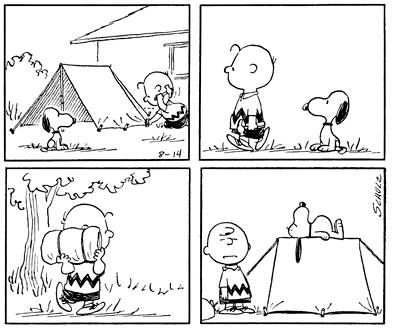
\includegraphics[scale=0.5]{comic-1.jpg}
    \end{center}
  \end{frame}

  \begin{frame}[t]{Le passé}
    Écris une histoire pour cette bande dessinée en utilisant \alert{l'imparfait} et \alert{le passé composé}.
    \begin{center}
      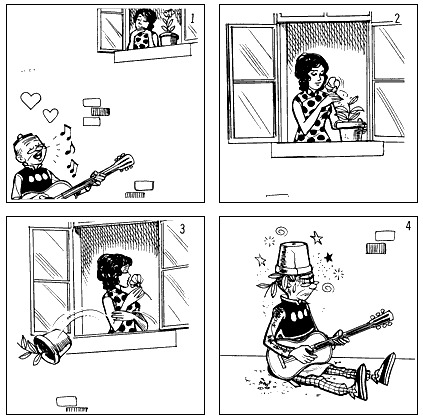
\includegraphics[scale=0.4]{comic-2.jpg}
    \end{center}
  \end{frame}

  \begin{frame}[t]{Le passé}
    Écris une histoire pour cette bande dessinée en utilisant \alert{l'imparfait} et \alert{le passé composé}.
    \begin{center}
      
\includegraphics[scale=0.55]{comic-3.jpg}
    \end{center}
  \end{frame}

  \begin{frame}{Les pronoms directs et indirects}
    \begin{enumerate}
      \item Dans le film d'action, Bond a envoyé \alert{un e-mail secret} au journaliste.
      \item<2->[$\to$] Bond l'a envoyé au journaliste.
      \item Il faut jeter les gobelets jetables \alert{dans le recyclage}.
      \item<3->[$\to$] Il faut y jeter les gobelets jeteables.
      \item Ces examens donnent de l'anxiété \alert{aux étudiants}.
      \item<4->[$\to$] Ces examens leur donnent de l'anxiété.
      \item Tu sais acheter \alert{les billets} à la machine?
      \item<5->[$\to$] Tu sais les acheter à la machine?
      \item Ils ont prêté des motos \alert{à Stéfanie} pour aller au spectacle.
      \item<6->[$\to$] Ils lui ont prêté des motos pour aller au spectacle.
      \item Est-ce que vous êtes libre pour venir \alert{à la maison} demain?
      \item<7->[$\to$] Est-ce que vous êtes libre pour y venir demain?
    \end{enumerate}
  \end{frame}

  \begin{frame}{Les pronoms relatifs}
    Il faut le pronom \lexi{qui}, \lexi{que} ou \lexi{où}?
    \begin{enumerate}
      \item Je lui ai offert un cadeau \underline{\uncover<2->{qui}} est tout neuf.
      \item Elle a rangé dans la cuisine ce cadeau \underline{\uncover<3->{que}} son voisin possède aussi.
      \item C'est un orage \underline{\uncover<4->{qui}} nous fait peur en hiver.
      \item Mon amie et moi ferons de la voile au lac \underline{\uncover<5->{où}} le ciel est tout le temps bleu.
      \item Jasper tenait son billet pour le moment \underline{\uncover<6->{où}} il faudra le donner au guide.
      \item Le guide nous a dit qu'il s'intéressait à la femme \underline{\uncover<7->{qu'}}on voyait dans le théâtre romain dans le passé.
    \end{enumerate}
  \end{frame}

  \begin{frame}{Écriture}
    \begin{enumerate}
      \item À l'avenir, tu auras un château et beaucoup d'argent. Sur un papier, décris le château en utilisant \alert{le futur proche} et \alert{le futur simple}. Décris les salles, les étages, l'extérieur, etc.
      \item<2-> Échange ta description avec la description d'un/e partenaire. Lis la description et note des erreurs potentielles \gloss{potential errors (things that might be errors)}.
      \item<3-> Rends la description à ton/ta partenaire, et discutez des notes.
    \end{enumerate}
  \end{frame}
\end{document}
